\documentclass[prd,aps,amsfonts,amsmath, nofootinbib]{revtex4}
\input{epsf}
\usepackage{graphicx}
\usepackage{thumbpdf}
%\usepackage{pdfsync}
%\usepackage[pdftex]{graphicx}


\def\be{\begin{equation}}
\def\en{\end{equation}}
\def\bea{\begin{eqnarray}}
\def\ena{\end{eqnarray}}

\begin{document}
\title{Preliminary evaluation of MLDC SMBH challenge: Round 1}
\author{S. Babak, E. Porter, M. Vallisneri}
\maketitle

\section{Challenge evaluation}

Three collaborations have submitted results for the challenge 1.2.1. Two submissions contain estimation of all nine parameters and the third one contains estimation of only chirp mass and time of coalescence.  We have only one entry for challenge 1.2.2.

In order to evaluate the results we have computed several quantities.  The noise weighted inner products were computed using the $X$-stream (used in MLDC) and two orthogonal streams with equal and uncorrelated noise:

\bea
A = (2X - Y - Z)/3; \;\;\;\; E = (Z - Y)/\sqrt{3}
\ena
and an approximate expression for the noise \bea
S = 2(S_X - S_{XY})/3
\ena
where for the frequency response used in synthetic LISA:
\bea
S_X &=& 16 \sin^2(2\pi fL)  (2 (1 + \cos^2(2\pi fL)) S_{pm} + S_{op})\\
S_{XY} &=& -4 \sin(4\pi fL)\sin(2\pi fL)  ( S_{op} + 4S_{pm} )\\
S_{pm} &=& 2.5\times10^{-48} \left(1 + \left(\frac{f}{10^{-4}Hz}\right)^{-2}
\right)  \left(\frac{f}{1Hz}\right)^{-2},\;\;\;
S_{op} = 1.8\times 10^{-37}  \left(\frac{f}{1Hz}\right)^2
\ena
We have computed the following quantities. The $\chi^2$ per degree
of freedom
\bea
\chi^{2} = \frac{(A_{data}- A_{rec}|A_{data}- A_{rec}) + 
(E_{data} - E_{rec}|E_{data} - E_{rec})}
{N-D}
\ena
and another (similar) quantity

\bea
\xi = \frac{\sqrt{(A_{data}- A_{rec}|A_{data}- A_{rec})^2 + 
(E_{data} - E_{rec}|E_{data} - E_{rec})^2}}
{N-D}
\ena
where $N$ is a number of data points and $D=9$ is number of parameters.

The next value is recovered combined SNR:
\bea
SNR  = \sqrt{SNR_A^2 + SNR_E^2},\\
SNR_A = \frac{(A_{data}|A_{rec})}{\sqrt{(A_{rec}|A_{rec})}},\;\;\;
SNR_E= \frac{(E_{data}|E_{rec})}{\sqrt{(E_{rec}|E_{rec})}}
\ena
Together with this we also compare the noiseless injected signal with 
the recovered one. Here we compute several overlaps:
\bea
O_A = \frac{(A_{key}|A_{rec})}{\sqrt{(A_{rec}|A_{rec})(A_{key}|A_{key})}}, \;\; 
O_E = \frac{(E_{key}|E_{rec})}{\sqrt{(E_{rec}|E_{rec})(E_{key}|E_{key})}}
\ena
and the overlap of the difference between the $X$ channels:
\be
O_{dX} = \frac{(X_{rec}-X_{key}|X_{rec}-X_{key})}
{\sqrt{(X_{rec}|X_{rec})(X_{key}|X_{key})}}
\en
The overlaps show how well we track the phase neglecting the error in 
the amplitude.

In order to take into account the possible error in the initial 
phase we have also computed overlaps maximized over the phase:

\bea
max_{\phi_0}(O_X) = \sqrt{(X_{rec}|X_{key}(\phi_0 = 0))^2 +
(X_{rec}|X_{key}(\phi_0 = \pi/2))^2}\\
min_{\phi_0}(O_{dX}) = \frac{ (X_{rec}|X_{rec}) + (X_{key}|X_{key}) -
2 max_{\phi_0}(X_{rec}|X_{key})}{\sqrt{(X_{rec}|X_{rec})(X_{key}|X_{key})}}
\ena

We have also computed the errors in the parameter estimations in units 
of $\sigma_{F}$, where $\sigma_{F}$ was taken from the square root of the diagonal elements of the covariance matrix (i.e. inverse of the Fisher matrix). These error estimates from the Fisher matrix were also checked against the LISA calculator.  Finally we plot the noiseless data and provide a visual comparison of the recovered signals against the key.

\section{Challenge 1.2.1}

We denote three entries as Montana/AEI, JPL, Goddard.
The results of computing various inner products are summarized in the 
Table~\ref{OlapsTable1.2.1}. The Montana/AEI entry has a constant phase difference (which is clear from values of
maximized overlaps), we have added one more entry (Montana/AEI*) with corrected initial phase.

\begin{table}
\caption{\label{OlapsTable1.2.1} Inner products for challenge 1.2.1}
\begin{ruledtabular}
\begin{tabular}{|c|c|c|c|c|c|c|c|c|}
Entry & $\chi^2$ & $\xi$ & SNR & $O_A$ & $O_E$ & $O_{dX}$ & $min_{\phi_0}(O_{dX})$ & $max_{\phi_0}(O_X)$\\
\hline
Key & 0.5824 & 0.41182 & 667.734 &  -- & -- & -- & -- & -- \\
Montana/AEI & 0.67193 & 0.47606 & 528.023 & 0.79153 & 0.79051 &
0.41694 & 0.000128 & 0.99994\\
JPL & 0.58451 & 0.41331 & 664.471 & 0.9944 & 0.9958 & 0.0112 &  0.00909 & 0.9955\\
Montana/AEI* & 0.58331 & 0.412466 & 666.324 & 0.998 & 0.998 & 0.0112 & 0.000128 & 0.99994 \\
\hline
\end{tabular}
\end{ruledtabular}
\end{table}

The 9-d covariance matrix for the parameter set $\vec{x}=\{\ln(M_{c}), \ln(\mu), \ln(D_{L}), \theta_{CL}, \phi, \iota, \psi, \ln(t_{c}), \varphi_{c}\}$ evaluated with the key file is given by
\be
\left( \begin{array}{ccccccccc}
 %3.872372e-10  &   5.487736e-09 &   -4.830902e-08 &  -6.512430e-09 &  3.874956e-09  &  -2.797328e-08  & -1.947460e-08   & 6.921398e-12  &  6.832675e-07\\
 %5.487736e-09   &  8.895662e-08  &  -4.304437e-07  &  1.219430e-08 & -6.682858e-08  &  -7.488979e-08  &  3.690754e-07   1.161215e-10   & 1.401720e-05\\
%-4.830902e-08  &  -4.304437e-07   &  3.040359e-04 &   1.676021e-05 &  7.627013e-06  &   1.280722e-04 &  -1.853579e-05  -6.568543e-12  & -1.714562e-05\\
%-6.512430e-09  &   1.219430e-08  &   1.676021e-05  &  3.293878e-06 & -2.384544e-06  &   1.123548e-05  &  1.171880e-05  -1.322383e-11  &  4.981729e-05\\
% 3.874956e-09  &  -6.682858e-08  &   7.627013e-06  & -2.384544e-06 &  4.513706e-06  &  -2.712281e-06 &  -1.819819e-05   2.635738e-11   &-7.240383e-05\\
%-2.797328e-08  &  -7.488979e-08  &   1.280722e-04  &  1.123548e-05 & -2.712281e-06  &   6.417406e-05  &  2.222767e-05   %7.460451e-12   & 1.138302e-04\\
%-1.947460e-08  &   3.690754e-07  &  -1.853579e-05  &  1.171880e-05 & -1.819819e-05  &   2.222767e-05  &  9.518923e-05   5.743921e-11   & 3.779646e-04\\
% 6.921398e-12  &   1.161215e-10  &  -6.568543e-12  & -1.322383e-11 &  2.635738e-11  &   7.460451e-12 &   5.743921e-11   1.707089e-13   & 1.785465e-08\\
% 6.832675e-07  &   1.401720e-05  &  -1.714562e-05  &  4.981729e-05 & -7.240383e-05  &   1.138302e-04  &  3.779646e-04   1.785465e-08   & 3.398534e-03
 3.87e-10  &   5.49e-09 &   -4.83e-08 &  -6.51e-09 &  3.87e-09  &  -2.8e-08  & -1.95e-08   & 6.92e-12  &  6.84e-07\\
 5.49e-09   &  8.9e-08  &  -4.30e-07  &  1.22e-08 & -6.68e-08  &  -7.49e-08  &  3.69e-07 &  1.16e-10   & 1.40e-05\\
-4.83e-08  &  -4.30e-07   &  3.04e-04 &   1.68e-05 &  7.63e-06  &   1.28e-04 &  -1.85e-05 & -6.57e-12  & -1.71e-05\\
-6.51e-09  &   1.22e-08  &   1.68e-05  &  3.29e-06 & -2.38e-06  &   1.12e-05  &  1.17e-05 & -1.32e-11  &  4.98e-05\\
 3.87e-09  &  -6.68e-08  &   7.63e-06  & -2.38e-06 &  4.51e-06  &  -2.71e-06 &  -1.82e-05 &  2.63e-11   &-7.24e-05\\
-2.8e-08  &  -7.49e-08  &   1.28e-04  &  1.12e-05 & -2.71e-06  &   6.42e-05  &  2.22e-05  & 7.46e-12   & 1.14e-04\\
-1.95e-08  &   3.69e-07  &  -1.85e-05  &  1.17e-05 & -1.82e-05  &   2.22e-05  &  9.52e-05 &  5.74e-11   & 3.78e-04\\
 6.92e-12  &   1.16e-10  &  -6.57e-12  & -1.32e-11 &  2.63e-11  &   7.46e-12 &   5.74e-11 &  1.71e-13   & 1.79e-08\\
 6.83e-07  &   1.40e-05  &  -1.71e-05  &  4.98e-05 & -7.24e-05  &   1.14e-04  &  3.78e-04 &  1.79e-08   & 3.4e-03
\end{array}
\right)
\en
%Note that off diagonal elements represented by correlation with actual parameters, not $\ln$ ({\bf Ed please confirm it}).
%This corresponds to the following values of one sigma deviation for a given in challenge 1.2.1 parameter set:
The variance-covariance matrix provides us with the following values for a 1-$\sigma$ error in the parameter estimation

\bea
M_c &=& 1.208590\times 10^6,\;\;\;     \sigma = 23.78306\\
\mu &=& 5.811961\times 10^5,\;\;\;     \sigma = 173.3452\\
D_{L} &=& 8.000000,\;\;\;     \sigma = 0.1394930\\
\theta_{CL} &=& 2.063085, \;\;\;   \sigma = 0.0018149\\
\phi &=& 0.865777 , \;\;\;      \sigma = 0.00212455\\
\iota &=& 1.94439 , \;\;\;       \sigma = 0.00801087\\
\psi &=& 3.23422, \;\;\;        \sigma = 0.0097565\\
t_{c} &=& 1.337403\times 10^7,\;\;    \sigma = 5.525738\\
\varphi_{c} &=& 4.364670, \;\;\;      \sigma = 0.058297
\ena

Note that in the above list,  the latitude has been converted to co-latitude according to $\theta_{CL}=\pi/2 - \theta_{L}$, luminosity distance and its error are quoted in Gpc, all angles are in radians, $t_{c}$ is quoted in seconds and we transform from initial orbital phase to gravitational wave phase at coalescence according to $\varphi_{c} = 2\left(\Phi_{0}-\phi(\omega(t=0))\right)$, where $\omega(t=0)$ is the orbital frequency evaluated at $t=0$.  

The errors in the parameter estimation (in units of sigma) are presented in the Table~\ref{Errors1.2.1}
\begin{table}
\caption{\label{Errors1.2.1} Errors in estimation of parameters for challenge 1.2.1. Values in brackets corresponds to the 
opposite direction on the sky.}
\begin{ruledtabular}
\begin{tabular}{|c|c|c|c|c|c|c|c|c|c|}
Entry & $\Delta M_c$ & $\Delta \mu $ & $\Delta D_{L}$ & $\Delta \theta $ & $\Delta \phi $ & $\Delta \iota $ &
$\Delta \psi $ & $\Delta t_c $& $\Delta \varphi_c $ \\ 
\hline
 JPL & 37.3& 36.8 &-63.2 & 566.308 (23.75)& -1493.76  (-15.08) & 165.719 & -271.752 & -8.1 &
0.074\\
Montana/AEI & -5.0 & -3.5 & 2.4  & 0.63 & 0.63 & 2.1 & 322.0 & -0.62 &  0.076 \\
Goddard & -2203 & -- & --  & --& -- & -- & -- & -- & -1433 \\
\hline
\end{tabular}
\end{ruledtabular}
\end{table}


Finally in Figure~\ref{fig1.2.1} we compare the beginning and the end of the recovered signals as compared to the signals generated using the key file. 
\begin{figure}[ht]
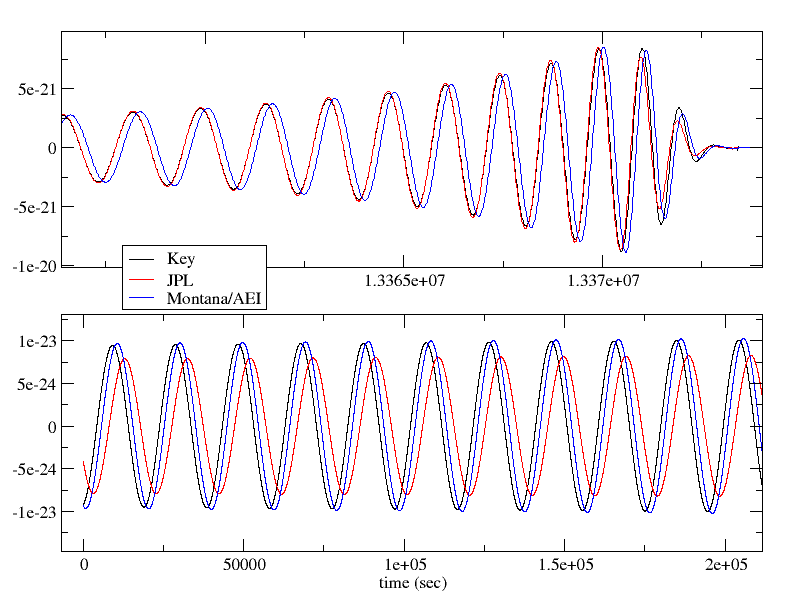
\includegraphics[height=0.6\textheight,
keepaspectratio=true,angle=0]{1_2_1X}
\caption{Comparison of the $X$-response to the signal from inspiralling SMBH. }
\label{fig1.2.1}
\end{figure}

The JPL signal provides a very good fit to the key in the LISA's most sensitive frequency band, but not across the whole bandwidth.  We can see however from Table II that even though there is a large error in the estimation of parameters for the JPL entry, the combination of these parameters results in a waveform that matches  the key-file waveform extremely well at end of the waveform where most of the SNR is accumulated.  The Montana/AEI waveform matches the amplitude and phase of the key-file signal extremely well throughout the entire bandwidth (except for the constant phase offset which has since been attributed to a missing sign allocation in the code).  When we maximize over phase we can see that the Montana/AEI overlaps truely reflect the close parameter estimation. 

 
\section{Challenge 1.2.2}

There is only one entry for this challenge. Here we again present the inner product and parameter estimation results, which are summarized in Table~\ref{OlapsTable1.2.2} and Table~\ref{Errors1.2.2}.  Again note that the errors for luminosity distance are given in Gpc, the error for $t_{c}$ is given in seconds and the angular errors are in radians.

\begin{table}
\caption{\label{OlapsTable1.2.2} Inner products for challenge 1.2.2}
\begin{ruledtabular}
\begin{tabular}{|c|c|c|c|c|c|c|c|c|}
Entry & $\chi^2$ & $\xi$ & SNR & $O_A$ & $O_E$ & $O_{dX}$ & $min_{\phi_0}(O_{dX})$ & $max_{\phi_0}(O_X)$\\
\hline
Key & 0.58063 & 0.410566 & 106.77 & -- & -- & -- & -- & -- \\
Montana/AEI & 0.58064 & 0.41058 &  106.60 & 0.9984 & 0.9987 & 0.0033 & 0.0029 & 0.9985 \\
\hline
\end{tabular}
\end{ruledtabular}
\end{table}

\begin{table}
\caption{\label{Errors1.2.2} Errors in estimation of parameters for challenge 1.2.2. }
\begin{ruledtabular}
\begin{tabular}{|c|c|c|c|c|c|c|}
Entry & $\Delta M_c$ & $\Delta \mu $ & $\Delta D_{L}$ & $\Delta \theta $ & $\Delta \phi $ & $\Delta t_c $ \\ 
\hline
$\sigma_{F}$ & 97.78 & 5,273 & 8.682 & 0.00507 & 0.00527 & 2,827\\
Montana/AEI & -2.35 & -2.66 & 0.125  & 3.728 & 1.025 & -2.33  \\
\hline
\end{tabular}
\end{ruledtabular}
\end{table}


The visual comparison (again beginning and end of the waveform) is presented in the figure~\ref{fig1.2.2}.  We can see in this case the phase and amplitude from the recovered signal match the key-file signal almost perfectly.

\begin{figure}[ht]
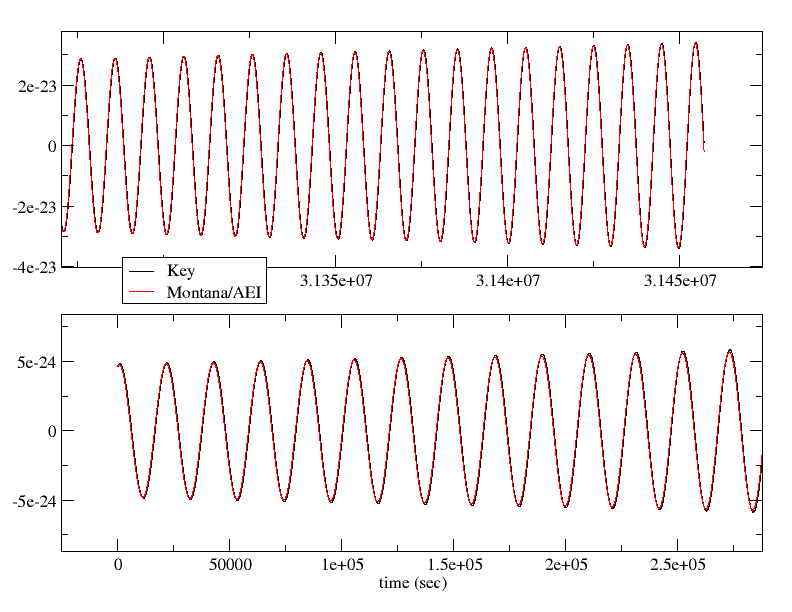
\includegraphics[height=0.6\textheight,
keepaspectratio=true,angle=0]{Eval122.png}
\caption{Comparison of the $X$-response to the signal from inspiralling SMBH. }
\label{fig1.2.2}
\end{figure}

\end{document}
